\documentclass[14pt, a4paper, ukrainian]{extreport}

\usepackage[14pt]{extsizes}
\usepackage{cmap}
\usepackage[utf8]{inputenc}
\usepackage[T2A]{fontenc}
\usepackage[english, ukrainian]{babel}
\usepackage{slashbox}
\usepackage{caption}
\DeclareCaptionLabelFormat{gostfigure}{Рисунок #2}
\DeclareCaptionLabelFormat{gosttable}{Таблиця #2}
\DeclareCaptionLabelSeparator{gost}{~---~}
\captionsetup{labelsep=gost}
\captionsetup*[figure]{labelformat=gostfigure}
\captionsetup*[table]{labelformat=gosttable}
\captionsetup*[figure]{labelformat=gostfigure, justification=centering}  % выравнивание по центру



\usepackage{titlesec}

\titleformat{\chapter}[block]
{\filcenter}
{\thechapter}
{1em}
{\MakeUppercase}
{}

\titlespacing*{\chapter}{0pt}{-40pt}{*4} 

\titleformat{\section}
{\filright}
{\thesection}
{1ex}{}

\titleformat{\subsection}
{\filright}
{\thesubsection}
{1ex}{}

%Clickable contents list
\usepackage{hyperref}
\hypersetup{
	pdftitle={Розрахунково-графічна робота},
	pdfauthor={Олександр Вергелюк},
	linkbordercolor= 1 1 1
}




\title{Розрахунково-графічна робота}
\author{Олександр Вергелюк}
\date{\today}


\usepackage[left=3.00cm, right=1.50cm, top=2.00cm, bottom=2.00cm]{geometry}

%Робота з математикою 
\usepackage{graphicx}
\usepackage{amsmath, amsfonts, amssymb, mathtools} %AMS
\usepackage{icomma} %Розумна кома
\usepackage{indentfirst}
\parindent 1.25cm
\usepackage[usenames,dvipsnames]{color}
\usepackage{makecell}
\usepackage{multirow}
\usepackage{ulem}
\usepackage{float}

%Шрифти
\usepackage{euscript}
\usepackage{mathrsfs}
\linespread{1.3} % полуторный интервал

\begin{document}
	\begin{titlepage}
		\centering
		\vspace{1cm}
		{ МІНІСТЕРСТВО ОСВІТИ І НАУКИ УКРАЇНИ\\
			НАВЧАЛЬНО-НАУКОВИЙ КОМПЛЕКС\\
			``ІНСТИТУТ ПРИКЛАДНОГО СИСТЕМНОГО АНАЛІЗУ``\\
			НАЦІОНАЛЬНОГО ТЕХНІЧНОГО УНІВЕРСИТЕТУ УКРАЇНИ\\
			``КИЇВСЬКИЙ ПОЛІТЕХНІЧНИЙ ІНСТИТУТ ІМЕНІ ІГОРЯ СІКОРСЬКОГО``\\
			КАФЕДРА МАТЕМАТИЧНИХ МЕТОДІВ  СИСТЕМНОГО АНАЛІЗУ\\\par}
		\vspace{5cm}
		\MakeUppercase {\textsc{\textbf{{розрахунково-графічна робота №2}}}}\\
		{з математичної статистики} \\
		\vfill
		\newlength{\ML}
		\settowidth{\ML}{\hspace{3.4cm}}
		\hfill
		\begin{minipage}{0.35\textwidth}
			Виконав студент 2 курсу групи КА-06\\
			Вергелюк Олександр\\ Андрійович
			
			Перевірив: \\
			Ільєнко Андрій\\ Борисович
		\end{minipage}
		\vfill
		\begin{center}
			Київ --- 2022
		\end{center}
	\end{titlepage}
	\setcounter{page}{2}
	\renewcommand\contentsname{Зміст}
	\tableofcontents
	\chapter*{Вступ}
	\addcontentsline{toc}{chapter}{Вступ}
	У файлі svyato.txt знайти свій набір із 100 чисел. Вони імітують вибірку, отриману із генеральної сукупності.
	
	\begin{center}
		Дана вибірка \linebreak
		
		\begin{tabular} {c c c c c c c c c c}
			-3.47 & 0.06 & -1.11 & -3.77 & 1.13 & 2.23 & -3.51 & -3.2 & -0.64 & -1.61 \\ 
			0.06 & -1.11 & -3.77 & 1.13 & 2.23 & -3.51 & -3.2 & -0.64 & -1.61 & -2.44 \\ 
			-1.11 & -3.77 & 1.13 & 2.23 & -3.51 & -3.2 & -0.64 & -1.61 & -2.44 & -5.44 \\ 
			-3.77 & 1.13 & 2.23 & -3.51 & -3.2 & -0.64 & -1.61 & -2.44 & -5.44 & -0.6 \\ 
			1.13 & 2.23 & -3.51 & -3.2 & -0.64 & -1.61 & -2.44 & -5.44 & -0.6 & 1.94 \\ 
			2.23 & -3.51 & -3.2 & -0.64 & -1.61 & -2.44 & -5.44 & -0.6 & 1.94 & -2.46 \\ 
			-3.51 & -3.2 & -0.64 & -1.61 & -2.44 & -5.44 & -0.6 & 1.94 & -2.46 & -1.12 \\ 
			-3.2 & -0.64 & -1.61 & -2.44 & -5.44 & -0.6 & 1.94 & -2.46 & -1.12 & -3.85 \\ 
			-0.64 & -1.61 & -2.44 & -5.44 & -0.6 & 1.94 & -2.46 & -1.12 & -3.85 & -1.0 \\ 
			-1.61 & -2.44 & -5.44 & -0.6 & 1.94 & -2.46 & -1.12 & -3.85 & -1.0 & -1.18 
		\end{tabular}
	\end{center}
	
	\begin{center}
		Відсортована вибірка \linebreak
		
		\begin{tabular} {c c c c c c c c c c}
		 -6.78 & -6.57 & -5.48 & -5.44 & -5.21 & -5.08 & -4.49 & -4.37 & -4.36 & -4.11 \\
		 -3.98 & -3.97 & -3.92 & -3.85 & -3.77 & -3.6 & -3.51 & -3.49 & -3.47 & -3.44 \\
		 -3.43 & -3.34 & -3.22 & -3.2 & -3.18 & -3.09 & -3.05 & -2.99 & -2.96 & -2.84 \\
		 -2.75 & -2.73 & -2.48 & -2.46 & -2.45 & -2.44 & -2.34 & -2.1 & -1.99 & -1.96 \\
		 -1.95 & -1.94 & -1.91 & -1.91 & -1.91 & -1.78 & -1.74 & -1.64 & -1.63 & -1.61 \\
		 -1.55 & -1.5 & -1.48 & -1.39 & -1.34 & -1.29 & -1.18 & -1.15 & -1.12 & -1.11 \\
		 -1.08 & -1.02 & -1.0 & -0.91 & -0.85 & -0.76 & -0.71 & -0.64 & -0.6 & -0.49 \\
		 -0.48 & -0.46 & -0.04 & -0.03 & 0.06 & 0.11 & 0.12 & 0.16 & 0.21 & 0.31 \\
		 0.32 & 0.4 & 0.44 & 0.87 & 0.99 & 1.05 & 1.13 & 1.16 & 1.18 & 1.24 \\
		 1.28 & 1.32 & 1.86 & 1.94 & 2.1 & 2.23 & 2.26 & 2.48 & 3.28 & 3.52
	\end{tabular}
	\end{center}

	Постановка задачі:
	
	\begin{enumerate}
		\item Проведіть первинний аналіз вибірки. Ци включає статистичний ряд (для неперервних розподілів --- інтервальний), емпіричну функцію розподілу (для неперервних розподілів --- інтервальну), її графік, полігон частот (для дискретних розподілів), гістограму (для неперервних розподілів), box-and-whisker plot.
		
		\item Знайдість вибіркове середнє, вибіркову дисперсію, виправлену вибіркову дисперсію, вибіркову медіану, вибіркову моду, вибіркові коефіцієнти асиметрії та ексцесу.
		
		\item \underline{Обґрунтуйте} та висуньте (нову) гіпотезу про розподіл генеральної сукупності.
		
		\item Методом моментів та методом максимальної вірогідності знайдіть оцінки параметрів розподілу. В деяких випадках це може бути не дуже просто (як, наприклад, для параметру \textit{N} біноміальної генеральної сукупності). Це чудовий спосіб проявити креативність та/або вміння користуватися Google.
		
		\item Для кожного параметру кращу у цих двох оцінок перевірте на \break
		(асимптотичну) незміщеність, консистентність та ефективність. Тут також має сенс зауваження до попереднього пункту. У випадку \break нездоланних труднощів --- а це відноситься \underline{виключно} до перевірки ефективності \textit{a} та \textit{b} в U(\textit{a, b}), \textit{a} в Exp(\textit{y, a}) та \textit{N} в Bin(\textit{N, p}) --- відповідну перевірку можно пропустити.
		
		\item Побудуйте довірчі інтервали надійністю 0.95 для параметрів розподілу. (The above notes still apply!)		
		
		\item Нарешті перевірте висунуту гіпотезу про розподіл генеральної сукупності за допомогою критерію $\chi^2$. Якщо гіпотеза суперечить вибірковим даним, перейдіть до п.3.
		
		\item Проявiть всi свої лiтературнi здiбностi та напишiть висновки.
		
	\end{enumerate}

	Інструменти, що я використовував під час роботи над цією РГР:
	\begin{itemize}
		\item Jupyter notebook
	\end{itemize}
	
	\chapter{Первинний аналіз вибірки}
	
	З загального виду вибірки видно, що її переважну більшість становлять раціональні числа, серед яких лише одне значення повторюється. Отже, можна висунути припущення, що надана вибірка з неперервного розподілу генеральної сукупності. Подальший аналі вибірки буде наподитися для випадку неперервного розподілу.
	
	Побудуємо інтервальний ряд для вибірки. Для цього за формулою Стерджеса визначимо кількість інтервалів.
	$$N_{intervals} = 1 + 3.322 * \lg n \approx 8$$
	Тепер знайдемо розмах вибірки, щоб обрати довжини інтервалів.
	$$R = x_{(n)} - x_{(1)} = 3.52 - (-6.78) = 10.3$$
	
	Для зручності в подальшому оберемо однакові довжини для всіх інтервалів причому такі, щоб точки, які визначають межі інтервалів мали лише один знак після коми.
	$$h = \frac{R}{N_{intervals}} = \frac{10.3}{8} \approx 1.3$$
	Тепер можемо побудувати статистичний ряд, табл. \ref{tab:stats}.
	\begin{table}[H]
		\caption{\label{tab:stats} Інтервальний статистичний ряд}
		\begin{center}
			\begin{tabular}{| l | l | l | l | l | l |}
				\hline
				$\Delta_k$ 	 & $x_k^*$ & $n$ & $n^*$ & $\nu$ & $\nu^*$ \\
				\hline
				[-6.8 ;  -5.5) & -6.15 &   2 &     2 &  0.02 &    0.02 \\
				\hline
				[-5.5 ;  -4.2) & -4.85 &   7 &     9 &  0.07 &    0.09 \\
				\hline
				[-4.2 ;  -2.9) & -3.55 &  20 &    29 &   0.2 &    0.29 \\
				\hline
				[-2.9 ;  -1.6) & -2.25 &  21 &    50 &  0.21 &     0.5 \\
				\hline
				[-1.6 ;  -0.3) & -0.95 &  22 &    72 &  0.22 &    0.72 \\
				\hline
				[-0.3 ;   1.0) &  0.35 &  13 &    85 &  0.13 &    0.85 \\
				\hline
				[ 1.0 ;   2.3) &  1.65 &  12 &    97 &  0.12 &    0.97 \\
				\hline
				[ 2.3 ;   3.6] &  2.95 &   3 &   100 &  0.03 &     1 \\
				\hline
			\end{tabular}
		\end{center}
	\end{table}
	
	Тепер за статистичним рядом можна побудувати емпіричну інтервальну функцію розподілу.
	$$ F_n^*(x) =
	\begin{cases}
		0 & x \le -6.8\\
		0.02 & -6.8 < x \le -5.5\\
		0.09 & -5.5 < x \le -4.2\\
		0.29 & -4.2 < x \le -2.9\\
		0.5 & -2.9 < x \le -1.6\\
		0.72 & -1.6 < x \le -0.3\\
		0.85 & -0.3 < x \le 1\\
		0.97 & 1 < x \le 2.3\\
		1 & 2.3 < x \le 3.5\\
	\end{cases} 
	$$
	
	Графік цієї функції наведено на рис. \ref{im:distribution_func}.
	\begin{figure}[H]
		\centering
		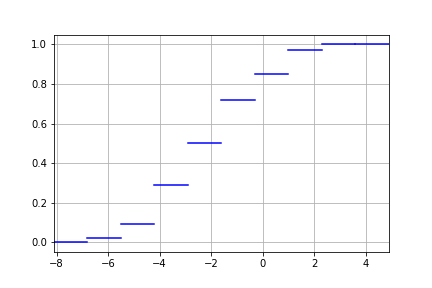
\includegraphics[width=0.8\textwidth]{./Image/CDF.png}
		\caption{Графік емпіричної інтервальної функції розподілу}
		\label{im:distribution_func}
	\end{figure}

	Гістограма для даної вибірки наведена на рис. \ref{im:hist}
	\begin{figure}[H]
		\centering
		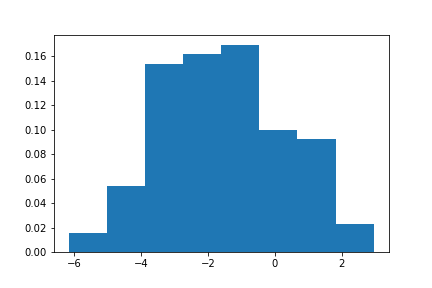
\includegraphics[width=0.8\textwidth]{./Image/Histogram.png}
		\caption{Гістограма даної вибірки}
		\label{im:hist}
	\end{figure}
	
	Тепер побудуємо діаграму box-and-whisker (ящик з вусами) для даної вибірки (рис. \ref{im:box_and_whisker}).
		\begin{figure}[H]
		\centering
		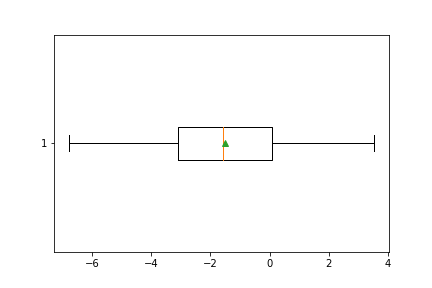
\includegraphics[width=0.8\textwidth]{./Image/Box_and_whisker.png}
		\caption{Box-and-whisker}
		\label{im:box_and_whisker}
	\end{figure}	
	
	\chapter{Описові стастики}
	Тепер знайдемо описові статистики вибірки: вибіркове середнє, вибіркову дисперсію, виправлену вибіркову десперсію, вибіркову медіану, мибіркову моду, вибіркові коефіцієнти асиметрії та ексцесу.
	
	Знайдемо вибіркове середнє:
	$$ \overline{x} = \frac{1}{n}\sum_{i=1}^{n}x_i = -1.5207$$
	
	Тепер обчислимо вибіркову дисперсію
	$$ \mathbb{D}\xi^{**} = \frac{1}{n}\sum_{i=1}^{n}(x_i - \overline{x})^2 = 4.5888$$
	
	Знайдемо виправлену вибіркову дисперсію
	$$ \mathbb{D}\xi^{***} = \frac{1}{n-1}\sum_{i=1}^{n}(x_i - \overline{x})^2 = 4.6352$$
	
	Оскільки в нашій вибірці n = 100, то медіана вибірки:
	$$ M_e^* = \frac{x_{(50)} + x_{(51)}}{2} = \frac{-1.61 - 1.55}{2} = -1.58$$
	
	Оскільки наша вибірка з неперервного розподілу генеральної сукупності, то вибіркова мода визначається за формулою:
	$$ M_o^* = y_{mo-1} + h \frac{n_i - n_{i-1}}{(n_i - n_{i-1}) + (n_i - n_{i+1})} = $$
	$$ = -1.6 + 1.3\frac{22 - 21}{(22 - 21) + (22 - 13)} = - 1.47$$

	Обчислимо вибірковий коефіцієнт асиметрії:
	$$ A_s = \frac{\overline{M_3}}{s_0^3} = \frac{\sum_{i=1}^{n}(x_i - \overline{x})^3}{ns_0^3} = 0.0318$$
	
	Знайдемо вибірковий коефіцієнт ексцесу:
	$$ E_k = \frac{\overline{M_4}}{s_0^4} - 3= \frac{\sum_{i=1}^{n}(x_i - \overline{x})^4}{ns_0^4} - 3 = -0.3145$$
		
	\chapter{Гіпотеза про розподіл генеральної сукупності}
	
	Оскільки з самого початку було прийнято припущення, що генеральна сукупність має неперервний розподіл, то логічно визначати можливий розподіл із неперервних. За умовою, це можуть бути 3 варіанти:
	\begin{itemize}
		\item гауссівський;
		\item рівномірний;
		\item експоненціальний із зсувом.
	\end{itemize}

	Візьмемо до уваги кілька фактів, які ми отримали при первинному аналізі вибірки.
	\begin{enumerate}
		\item Гістограма за виглядом дещо нагадує графік щільності розподілу гауссівського розподілу ("дзвін").
		\item Емпірична функція розподілу лише трохи нагадує функцію розподілу гаусівського розподілу, але зовсім трохи.
		\item За графіком box-and-whisker видно, що половина усіх значень вибірки лежить у відносно вузькому проміжку, який трохи менше за $\frac{1}{3}$ розмаху вибірки. Це схоже із правилом для гауссівського розподілу, коли в в межах одного стандартного відхилення від математичного сподівання лежить 68.26\% усіх значень. Це ще один аргумент на користь гауссівського розподілу.
		\item Вибіркове середнє (-1.52), вибірова мода (-1.47) та вибіркова медіана (-1.58) ці значення доволі близькі один до одного, що схоже на гауссівський розподіл, у якого ці значення мають співпадати.
	\end{enumerate}
	
	За сукупністю вище зазначених факторів приймемо гіпотезу $H_0$ --- вибірка з генеральної сукупності із гауссівським розподілом.
	
	\chapter{Оцінка параметрів розподілу}
	
	Відповідно до висунутої гіпотези $H_0$ знайдемо оцінки гауссівського розподілу $N (a, \sigma^2)$ знайдемо оцінки $a^*$ і $(\sigma^2)^*$ методом моментів та методом максимальної ймовірності. 
	
	\section{Метод моментів}
	
	За визначенням для гауссівського розподілу:
	$$a = \mathbb{E}\xi$$
	$$\sigma^2 = \mathbb{D}\xi$$
	
	Тоді оцінки розподілу будуть:
	$$ a_{MM}^* = \overline{\xi} \Rightarrow a_{MM}^* = -1.52$$
	$$ (\sigma^2)_{MM}^* = \mathbb{D}\xi^{**} \Rightarrow (\sigma^2)_{MM}^* = 4.6352$$
	
	Отже, маємо гауссівський розподіл $N (-1.52, 4.6352)$.
	
	\section{Метод максимальної правдоподібності}
	
	За методом максимальної правдоподібності:
	$$ \mathcal{L}(\vec{x}, a, \sigma^2)  = \prod_{k = 1}^{n} \frac{1}{\sigma\sqrt{2\pi}}e^{-\dfrac{(x_k - a)^2}{2\sigma^2}}$$
	$$ \ln\mathcal{L}(\vec{x}, a, \sigma^2)  = -\frac{n}{2} \ln 2\pi - \frac{n}{2}\ln \sigma^2 - \frac{1}{2\sigma^2}\sum_{k = 1}^{n}(x_k - a)^2$$
	
	Для знаходження максимуму функції від двох змінних запишимо систему:
	$$
	\begin{cases}
		\frac{\partial \ln \mathcal{L}}{\partial a}  = \frac{1}{\sigma^2}\sum_{k = 1}^{n}(x_k - a) = 0 \\
		\frac{\partial \ln \mathcal{L}}{\partial \sigma^2} = -\frac{n}{2\sigma^2} + \frac{1}{2\sigma^4}\sum_{k = 1}^{n}(x_k - a)^2 = 0
	\end{cases} 
	$$
	$$
	\begin{cases}
		\frac{1}{\sigma^2}n(\overline{x} - a) = 0 \\
		\frac{1}{2\sigma^4}\sum_{k = 1}^{n}(x_k - a)^2 = \frac{n}{2\sigma^2}
	\end{cases} 
	$$
	$$
	\begin{cases}
		\frac{n\overline{x}}{\sigma^2} = \frac{na}{\sigma^2} \\
		\frac{n}{2\sigma^4}\mathbb{D}x^{**} = \frac{n}{2\sigma^2}
	\end{cases} \Rightarrow
	\begin{cases}
		a^* = \overline{x} \\
		(\sigma^2)^* = \mathbb{D}x^{**}
	\end{cases} 
	$$
	Тепер знайдемо матрицю других похідних:
	$$ \left( \begin{matrix}
		\frac{\partial^2 \ln \mathcal{L}}{\partial a^2} & \frac{\partial^2 \ln \mathcal{L}}{\partial a \partial \sigma^2} \\
		\frac{\partial^2 \ln \mathcal{L}}{\partial \sigma^2 \partial a} & \frac{\partial^2 \ln \mathcal{L}}{\partial (\sigma^2)^2} \\
	\end{matrix} \right) = 
	\left( \begin{matrix}
		-\frac{n}{\sigma^2} &  -\frac{n}{\sigma^4}(\overline x - a)\\
		-\frac{n}{\sigma^4}(\overline x - a) & \frac{n}{2\sigma^4} - \frac{1}{\sigma^6}\sum_{k = 1}^{n}(x_k - a)^2\\
	\end{matrix} \right)
	$$
	
	При $a = a^*$ і $\sigma^2 = (\sigma^2)^*$:
	$$ \left( \begin{matrix}
		-\frac{n}{(\sigma^2)^*} & 0 \\
		0 & \frac{n}{((\sigma^2)^*)^3} \left(\frac{(\sigma^2)^*}{2}- \frac{1}{n}\sum_{k = 1}^{n}(x_k - a^*)^2 \right)\
	\end{matrix} \right)\ = 
	\left( \begin{matrix}
		-\frac{n}{(\sigma^2)^*} & 0 \\
		0 & -\frac{n}{2((\sigma^2)^*)^2} \\
	\end{matrix} \right)\
	$$
	
	Ця матриця є від'ємно визначеною, тому $\ln\mathcal{L}(\vec{x}, a, \sigma^2)$ дійсно досягає максимуму при $a = \overline{x}$ і $\sigma^2 = \mathbb{D}\xi^{**}$. Отже, отримали оцінки $a_{MMP}^* = \overline{\xi}$ та $(\sigma^2)_{MMP}^* = \mathbb{D}\xi^{**}$.
	
	Як бачимо, обома методами отримано однакові оцінки для параметрів даного розподілу: $a^* = \overline{\xi} = -1.52$ та $(\sigma^2)^* = \mathbb{D}\xi^{**} = 4.6352$.
	
	\chapter{Перевірка параметрів на незміщеність, консистентність та ефективність}
	
	Перевіримо отримані оцінки для кожного параметра на (асимптотичну) незміщеність, консистентність та ефективність. Нехай $\theta^*$ оцінка параметру $\theta$, тоді за означеннями:
	\begin{itemize}
		\item Незміщеність:
		$$ \mathbb{E}\theta_n^* = \theta \quad \forall n \in \mathbb{N}$$
		Асимптотично незміщеність:
		$$\lim_{n \to \infty}\mathbb{E}\theta_n^* = \theta$$
		\item Консистентність:
		$$\forall \varepsilon > 0: \lim_{n \to \infty} \mathbb{P} \{|\theta_n^* - \theta| \geq \varepsilon\} = 0 \Leftrightarrow \theta_n^* \xrightarrow{\mathbb{P}} \theta, n \to \infty$$
		\item Ефективність. Нехай $\Theta_n$ --- множина усіх незміщених оцінок параметру $\theta$ за вибірками фіксованого обсягу $n$. Оцінка $\theta_{\text{еф}}^*$ називається ефективною, якщо
		$$ \mathbb{D}\theta_n^* = \inf_{\theta^* \in \Theta_n}\mathbb{D}^*$$
		Зручно використовувати наступний критерій ефективності незміщеної оцінки (наслідок з нерівності Крамера-Рао):
		$$\frac{\partial \ln \mathcal{L}(\vec{\xi}, \theta)}{\partial \theta} = C(n, \theta)\cdot\left(\theta^*(\vec{\xi} - \theta)\right)$$
	\end{itemize}
	
	Як відомо, вибіркове середнє та вибіркова дисперсія консистентні оцінки, тому обидва параметра розподілу також консистентні, оскільки дорівнюють їм. 
	
	Вибіркове середнє --- незміщена оцінка, тоді оцінка параметру розподілу $a^* = \overline{\xi}$ --- незміщена оцінка. Вибіркова дисперсія --- асимптотично незміщена оцінка, тоді оцінка параметру розподілу $(\sigma^2)^* = \mathbb{D}\xi^{**}$ --- асимптотично незміщена. 
	
	Перевіримо оцінки на ефективність. Для оцінки параметру $a^* = \overline{\xi}$:
	$$\frac{\partial \ln \mathcal{L}(\vec{\xi}, a, \sigma^2)}{\partial a} = \frac{1}{\sigma^2}\sum_{k = 1}^{n}(x_k - a) = \frac{n}{\sigma^2}(\overline{\xi} - a) = C(n)\cdot(\overline{\xi} - a)$$
	Отже, можна зробити висновок, що оцінка параметру $a^* = \overline{\xi}$ --- ефективна.
	
	Оцінка параметру $(\sigma^2)^* = \mathbb{D}\xi^{**}$ лише асимптотично незміщена, тому не може бути ефективною.
	
	\chapter{Довірчі інтервали для параметрів розподілу}
	
	Побудуємо довірчі інтервали надійністю 0.95 для параметрів розподілу. 
	
	Для параметра $a$: $\mathbb{P} \{|a - a^*| < \varepsilon\} = 0.95$. Маємо:
	$$ \sqrt{n - 1} \frac{\overline{\xi} - a}{\sqrt{\mathbb{D}^{**}\xi}} \sim St_{n-1} $$
	З рівності
	$$\mathbb{P}\left\{\frac{\sqrt{n-1}|\overline{\xi} - a|}{\sqrt{\mathbb{D}^{**}\xi}} < t_\gamma\right\} = 0.95$$
	знайдемо $t_\gamma$.
	$$\frac{\sqrt{n-1}|\overline{\xi} - a|}{\sqrt{\mathbb{D}^{**}\xi}} < t_\gamma$$
	$$|\overline{\xi} - a| < \frac{t_\gamma\sqrt{\mathbb{D}^{**}\xi}}{\sqrt{n-1}}$$
	$$\overline{\xi} - \frac{t_\gamma\sqrt{\mathbb{D}^{**}\xi}}{\sqrt{n-1}} < a < \frac{t_\gamma\sqrt{\mathbb{D}^{**}\xi}}{\sqrt{n-1}} + \overline{\xi}$$
	
	$$\int_{t_{\gamma; n}}^{\infty}f(x)dx = \frac{1 - \gamma}{2} = \frac{1 - 0.95}{2} = 0.025$$
	
	Отже, треба знайти значення коєфіцієнта $t_{0.025; 99}$. В таблицях цей коефіцієнт не наводиться, найближчим є $t_{0.025; 100} = 1.984$. Візьмемо це значення за коефіцієнт $t_{0.025; 99} \approx 1.984$. Оскільки вибіркові статистики $\overline{\xi} = -1.5207$, a $\mathbb{D}^{**}\xi = 4.5888$. Тоді:
	$$\frac{t_\gamma\sqrt{\mathbb{D}^{**}\xi}}{\sqrt{n-1}} = \frac{1.984 \cdot \sqrt{4.5888}}{\sqrt{99}} = 0.4271$$

	Отже, $a \in (-1.9478; -1.0936)$.
	
	Для параметра $\mathbb{D}^**\xi$:
	$$\frac{n\mathbb{D}^**\xi}{\sigma^2} \in \chi_{n-1}^2$$
	Маємо:
	$$\frac{n\mathbb{D}^{**}\xi}{t_{\frac{1-\gamma}{2}}} < \sigma^2 < \frac{n\mathbb{D}^{**}\xi}{t_{\frac{1+\gamma}{2}}} $$
	
	$$\frac{1-\gamma}{2} = 0.025$$
	$$\frac{1+\gamma}{2} = 0.975$$
	Тоді беремо коефіцієнти $\chi^2_{0.025;99} \approx 129.6$ і $\chi^2_{0.975;99} \approx 74.22$.
	
	Межі довірчого інтервалу:
	$$\frac{n\mathbb{D}^{**}\xi}{t_{0.025; 99}} = 3.5407$$
	$$\frac{n\mathbb{D}^{**}\xi}{t_{0.975; 99}} = 6.1827$$
	
	Отже, $\sigma^2 \in (3.5407;6.1827)$.
	
	\chapter{Перевірка висунотої гіпотези за критерієм $\chi^2$}
	
	Перевіримо висунуту гіпотезу про розподіл генеральної сукупності за допомогою критерію $\chi^2$.
	
	Нехай $\xi \sim N(-1.5207,4.5888)$. Тоді побудуємо таблицю \ref{tab:kriteriy} для перевірки критерію $\chi^2$.
	
	\begin{table}[H]
		\caption{\label{tab:kriteriy} Таблиця для критерію $\chi^2$}
		\begin{center}
			\begin{tabular}{| l | l | l | l |}
				\hline
				$\Delta_k$ 	 & $n$ & $p_k = \mathbb{P}\left\{\xi \in \Delta_k\right\}$ & $np_k$\\
				\hline
				[-6.8 ;  -5.5) & 2 & 0.0252 & 2.52\\
				\hline
				[-5.5 ;  -4.2) & 7 & 0.0742 & 7.42\\
				\hline
				[-4.2 ;  -2.9) &  20 & 0.1555 & 15.55\\
				\hline
				[-2.9 ;  -1.6) &  21 & 0.2229 & 22.29\\
				\hline
				[-1.6 ;  -0.3) & 22 & 0.2317 & 23.17\\
				\hline
				[-0.3 ;   1.0) &  13 & 0.1653 & 16.53\\
				\hline
				[ 1.0 ;   2.3) &   12 & 0.0815 & 8.15\\
				\hline
				[ 2.3 ;   3.6] &   3 & 0.0293 & 2.93\\
				\hline
			\end{tabular}
		\end{center}
	\end{table}
	
	Як видно, умова $np_k \geq 10$ виконується не для всіх інтервалів, тому необхідно об'єднати деякі з них (табл. \ref{tab:kriteriy2}).
	
		\begin{table}[H]
		\caption{\label{tab:kriteriy2} Таблиця для критерію $\chi^2$}
		\begin{center}
			\begin{tabular}{| l | l | l | l |}
				\hline
				$\Delta_k$ 	 & $n$ & $p_k = \mathbb{P}\left\{\xi \in \Delta_k\right\}$ & $np_k$\\
				\hline
				[-6.8 ;  -2.9) &  29 & 0.2549 & 25.49\\
				\hline
				[-2.9 ;  -1.6) &  21 & 0.2229 & 22.29\\
				\hline
				[-1.6 ;  -0.3) & 22 & 0.2317 & 23.17\\
				\hline
				[-0.3 ;   1.0) &  13 & 0.1653 & 16.53\\
				\hline
				[ 1.0 ;   3.6] &   15 & 0.0815 & 11.08\\
				\hline
			\end{tabular}
		\end{center}
	\end{table}

	Тепер дослідимо величину 
	$$\chi^2(n) = \sum_{k = 1}^{m}\frac{(n_k - np_k)^2}{np_k} \sim \chi_{m-s-1}^2,$$
	де $m$ --- кількість інтервалів,\\
	$s$ --- кількість оцінених параметрів розподілу.
	
	В даному випадку $\chi_{m-s-1}^2 = \chi_2^2$, $\alpha = 0.05$, то треба взяти $\chi_{2;0.05}^2 =\\= 5.99$. Тепер обчислимо 
	$$\chi^2(n) = \sum_{k = 1}^{m}\frac{(n_k - np_k)^2}{np_k} = \sum_{k = 1}^{5}\frac{(n_k - np_k)^2}{np_k} = 2.758$$
	
	Як видно, $\chi^2(n) < \chi_{2; 0.05}^2$, то наявні дані не суперечать висунутій гіпотезі, тобто немає підстави відхилити запропоновану гіпотезу на рівні значущості 0.05.
	
	\chapter*{Висновки}
	\addcontentsline{toc}{chapter}{Висновки}
	
	В ході виконання розрахунково-графічної роботи було проаналізовано надану вибірку за допомогою широкого набору статистичних засобів. Спочатку проведено первинний аналіз даних та застосовано візуальні інструменти аналізу для отримання першої інтуїтивної гіпотези про клас розподілу генеральної сукупності. Гіпотеза полягала в тому, що генеральна сукупність розподілена за гауссівським розподілом. 
	
	На основі висунутої гіпотези про розподіл генеральної сукупності висунуто оцінки параметрів розподілу за допомогою методу моментів та методу максимальної правдоподібності. В обох випадках отримано оцінки $a^* = \overline{\xi}$ та $(\sigma^2)^* = \mathbb{D}^{**}\xi$. В подальшому дані оцінки перевірено на консистентність, (асимптотичну) незміщеність та ефективність. Оцінка параметру $a^* = \overline{\xi}$ має усі зазначені властивості, а оцінка $(\sigma^2)^* = \mathbb{D}^{**}\xi$ консистентна, асимптотично незміщена, але не ефективна.
	
	Для кожного параметру розподілу на основі отриманих оцінок побудовано довірчі інтервали з ймовірністю 0.95. В результаті отримано, що\break $a \in (-1.9478; -1.0936)$, а $\sigma^2 \in (3.5407;6.1827)$.
	
	В кінці виконано перевірку висунутої гіпотези про гауссівський розподіл генеральної сукупності за допомогою критерію $\chi^2$. В результаті визначено, що на рівні значущості 0.05 немає підстав відхилити початкову гіпотезу про гауссівський розподіл генеральної сукупності.
	
	
\end{document}